
In the previous chapter, we have explained the advantage of simple
zonotopes that they are closed under linear transformation and
Minkowski sum operations and these can be computed efficiently.
Regarding computation of a positive invariant real zonotope for a
linear system, we showed in Proposition~\ref{prop:eig-rztope} that it
can be done efficiently when the eigenvectors are real valued.
However, when the eigenvectors of a stable linear system are complex
valued, we can not guarantee the existence of a non-zero real
zonotopic positive invariant.  Overcoming this drawback of real
zonotopes, we extend them to a new class of sets called \emph{complex
zonotopes} by which we can easily specify positive invariants of a
stable linear system using the eigenstructure.  Henceforth, we believe
that even for affine hybrid systems, a complex zonotope can capture
contraction along the complex eigenvectors of some of the
transformation matrices.  Complex zonotopes are also geometrically
more expressive, since their real projections can describe some
non-polytopic sets as well as polytopic zonotopes.  Apart from
computing simple operations on complex zonotopes like linear
transformation and Minkowski sum, we shall derive a convex program for
checking inclusion between two complex zonotopes.  The inclusion
relation is a key ingredient for efficient invariant computation,
which we shall discuss in latter chapters.

This chapter is organized into three main sections.  In
Section~\ref{sec:representation}, we shall introduce the basic
representation of a complex zonotope that naturally extends the
Definition~\ref{defn:rztope} of real zonotopes.  Further on, we shall
introduce a more general but geometrically equivalent representation,
called \emph{template complex zonotope}, which allows efficient
modification of complex zonotopic sets for increasing accuracy of
abstraction of sets.  In Section~\ref{sec:operations-tcz}, we shall
discuss basic operations on a template complex zonotope like linear
transformation, Minkowski sum and computation of support function.  In
Section~\ref{sec:inclusion-tcz}, we shall derive a convex program for
checking the inclusion between two template complex zonotopes.  

\section{Representation of a complex zonotope}~\label{sec:representation}
The basic representation of a complex zonotope is a linear combination
of complex valued vectors with complex combining coefficients whose
absolute value is bounded by unity.  This is a generalization of the
representation of a simple zonotope given in Definition~\ref{defn:rztope} of
previous chapter to the space of complex numbers.  However, the real
projection of a complex zonotope is expressive because it can
represent some non-polyhedral sets in addition to the polyhedral
zonotopes, which we shall discuss later.
%
\begin{definition}[Complex zonotope]
Let $\ptemp\in\mat{m}{n}{\compnums}$ be a complex valued matrix
whose columns are called {\it generators} and $\cen\in\compnums^n$ be a
complex valued vector called the {\it center}.  The following is the
representation of a
complex zonotope.
%
\begin{equation}
\cztope{\ptemp}{\cen} := \set{\ptemp\zeta+\cen:~\zeta\in\compnums^m,~\infnorm{\zeta}\leq 1}.
\end{equation}
%
\end{definition}
%
{\it Geometry of a complex zonotope :}
The real projection of the set of points represented by each generator
can either be an ellipsoid or a line segment.  So, complex
zonotopes can represent a Minkowski sum of a some ellipsoids and line
segments.  Whereas, simple zonotopes represent only Minkowski sum of
line segments.  Therefore, complex zonotopes are geometrically more
expressive than real zonotopes.
For example, the real projection of the the following complex vector
is an ellipsoid.
%
\begin{align*}
& \cztope{\mymatrix{-0.1335 + 0.1769i\\0.2713 + 0.3991i\\-0.8473 + 0.0000i}}{0}:=~~\\
&  \lt(0.2749x-0.1218y+1.0978z\rt)^2+\lt(1.0505x+2.0401y+0.4877z\rt)^2\leq 1.
\end{align*}
%
On the other hand, the real projection of the following real vector, which is a
complex vector having zero imaginary part, is a line segment.
%
\begin{align*}
\cztope{\mymatrix{-0.4544\\
    0.7379\\
    0.4991}}{0}:=~~-1\leq -0.4544x+0.7379y+0.4991z\leq 1.
\end{align*}
%
The above observation is explained mathematically by the following
proposition, which describes the set formed by a single generator.  
%
\begin{proposition}
Let $v\in\compnums^n$ be a complex vector.  
%
\[
\real\lt(\cztope{v}{0}\rt)=\set{x\in\reals^n:\norm{\pinv{\mymatrix{\real(v)&\img{v}}}x}^2\leq
1}.
\]
%
The above set can either be an ellipsoid or a line segment.
\end{proposition}
%
\begin{proof}
Let us consider $x\in\cztope{v}{0}$.  Then there exists an
$\zeta\in\compnums$ such that $\absolute{\zeta}\leq 1$ and
$x=v\zeta$.  Then we derive the following.
%
\begin{align*}
& \min{\absolute{\zeta}:~\zeta\in\compnums,~x=v\zeta}\\
& =\min{\sqrt{a^2+b^2}:~a,b\in\reals,~x=\mymatrix{\real(v)
& \img\lt(v\rt)}\mymatrix{a\\b}}=\norm{\pinv{\mymatrix{\real(v)
& \img\lt(v\rt)}}x}.
\end{align*}
%
Therefore, $x\in\cztope{v}{0}$ implies $\norm{\pinv{\mymatrix{\real(v)
& \img\lt(v\rt)}}x}^2\leq 1$.
\end{proof}
%
%% The real projection of a complex
%% zonotope can represent non-polytopic sets as well as polytopic
%% zonotopes.  Therefore, complex zonotopes are geometrically more
%% expressive than simple zonotopes.  Furthermore, complex zonotopes are
%% different from polynomial zonotopes.  While a polynomial zonotope is a
%% polynomial function of real valued intervals, a complex zonotope is a
%% Minkowski sum of \emph{linearly transformed transformed circles} in
%% the the complex plane.  A complex zonotope is symmetric around the center.  To see
%%  this, consider a point in a complex zonotope centered at the origin,
%%  written as $y=\ptemp\zeta$ where $\ptemp$ defines the generator set
%%  and $\zeta$ is the vector of combining coefficients.  Since,
%%  $\infnorm{-\zeta}=\infnorm{\zeta}\leq 1$, so $-y=\ptemp(-\zeta)$ also
%%  belongs to the complex zonotope.

%% {\it Example: } The real projection of the complex zonotope
%% %
%% \[
%% \cztope{\mymatrix{(1+2i) & 1 & (2+i)\\(1-2i) & 0 & (2-i)}}{0}.
%% \]
%% %
%% is a Minkowski sum of two ellipses and one line segment as shown in
%%  Figure~\ref{fig:cz}.  It is symmetric around the origin.
  
%% %
%% \begin{figure}
%% \centering
%% \captionsetup{justification=centering}
%% 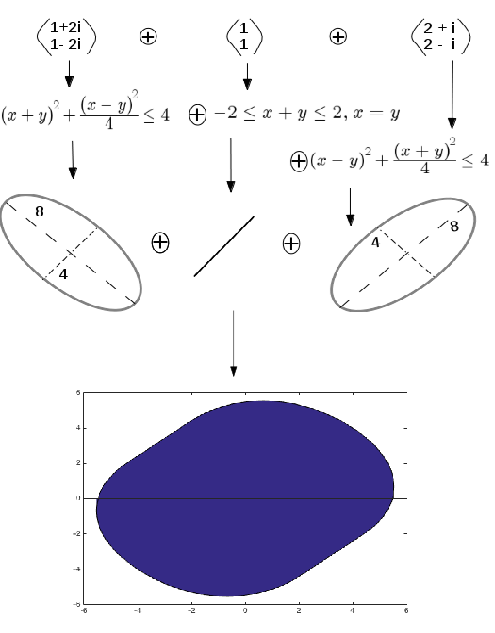
\includegraphics[scale=0.43]{fig/cznew.png}\\[1em]
%% 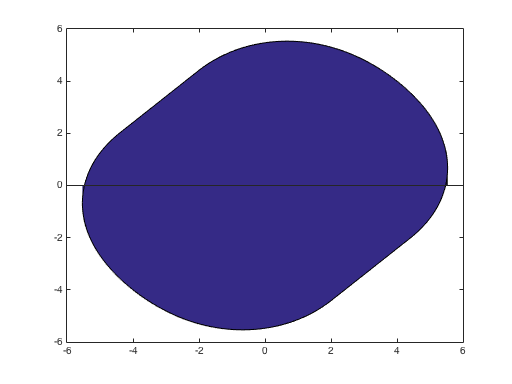
\includegraphics[scale=0.5]{fig/CZhull.png}
%% \caption{Real projection of a complex zonotope as\\ Minkowski sum of 2 ellipses and 1 line segment }~\label{fig:cz}
%% \end{figure}
%% %

As the real projection of the generator of a complex zonotope can
either be an ellipsoid or a line segment, a complex zonotope can
represent a Minkowski sum of line segments as well as some
ellipsoids.  The non-polyhedral real projections along the three axis
oriented hyperplanes of the following 3-D complex zonotope is shown in
Figure~\ref{fig:3dcztope}
%
\[
\cztope{\mymatrix{-0.2226  & -0.1335 + 0.1769\iota  & -0.1335 - 0.1769\iota\\
   0.3615 &   0.2713 + 0.3991\iota &  0.2713 - 0.3991\iota\\
   0.2446 &  -0.8473 &  -0.8473}}{0}
\]
%
\begin{figure}
\center
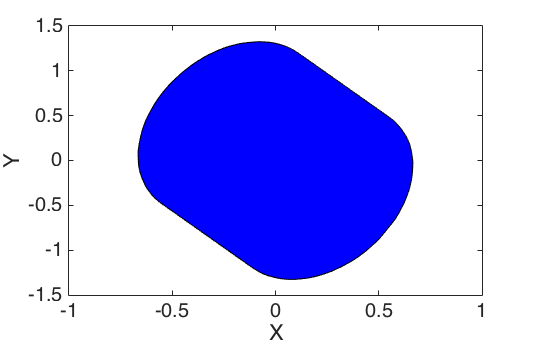
\includegraphics[scale=0.5]{fig/CZtopes/xycz.png}
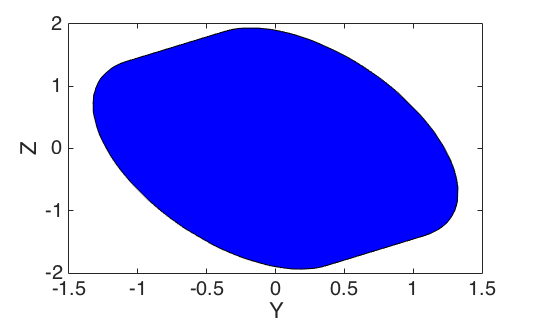
\includegraphics[scale=0.5]{fig/CZtopes/yzcz.png}
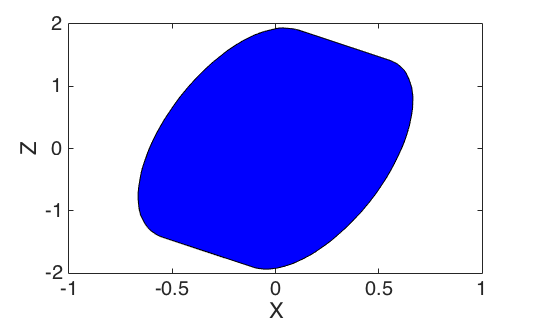
\includegraphics[scale=0.5]{fig/CZtopes/xzcz.png}
\caption{Real projection of complex zonotope on axis oriented hyperplanes}~\label{fig:3dcztope}
\end{figure}
%

\emph{Contraction along eigenvectors:  }  A motivation for extending
simple zonotopes to complex zonotopes is that a complex zonotope with
its generators as the complex eigenvectors of a discrete time linear
system is positively invariant if the complex eigenvalues
corresponding to the generators are bounded within unity in their
absolute values.  This is because the generators of the resultant
complex zonotope after transformation will be scaled by the absolute
values of the corresponding eigenvalues.  For example, consider the
following matrix $A$ and the complex zonotope
$\cztope{V}{0}$ generated by the complex eigenvectors of $A$.
%
\begin{align*}
& A=\mymatrix{
0.1502 &  -0.0438  &  0.1366\\
    0.7482 &   0.1470  &  0.1251\\
   -0.8436 &  -0.7027  &  0.0418
}\\
& V=\mymatrix{
-0.2226  &  -0.1335 + 0.1769\iota &  -0.1335 - 0.1769\iota\\
   0.3615 &   0.2713 + 0.3991\iota &  0.2713 - 0.3991\iota\\
   0.2446 & -0.8473 &   -0.8473 
}
\end{align*}
%
The eigenvalues of $A$ are $-0.2291$, $0.1339 + 0.5071\iota$ and
${0.1339 - 0.5071\iota}$, whose absolute values are $0.2291$,
$0.5245$, and $0.5245$, respectively.  After the transformation by
$A$, the set generated by $V^T_1$ gets scaled down to $0.2291$ times
its size and that of $V^T_2$ and $V^T_3$ to $0.5245$ times
its their size.  So, the complex zonotope, which is a Minkowski sum
of these sets, contracts after the transformation.  This is illustrated
in Figure~\ref{fig:cz-scaled-down}, which shows the contraction of
each of the sets formed by the generators and the consequent
contraction of the complex zonotope.
%
\begin{figure}
\center
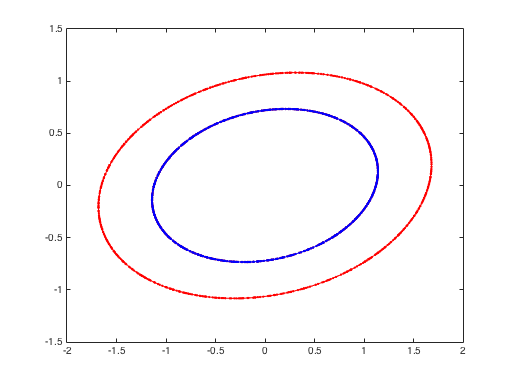
\includegraphics[scale=0.4]{fig/CZtopes/eigcontraction.png}
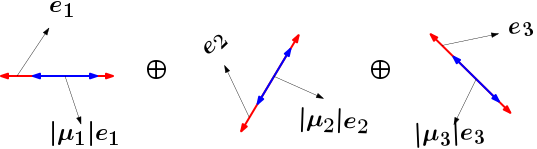
\includegraphics[scale=0.5]{fig/CZtopes/contraction-zonotope.png}
\caption{Contraction of complex zonotope along
eigenvectors}~\label{fig:cz-scaled-down}
\end{figure}
%
This property of contraction of complex zonotope by a linear
transformation based on the eigenstructure of a matrix is explained
mathematically in the following proposition.
%
\begin{proposition}[Eigenstructure based invariance]~\label{lem:eig-invariance}
Let us consider $\ptemp\in\mat{n}{n}{\compnums}$ consists of the
complex eigenvectors of a matrix $A\in\mat{n}{n}{\reals}$ as its
column vectors and $\mu\in\compnums^n$ be the vector of complex
eigenvalues, i.e., $A\ptemp = \ptemp\diagonal{\mu}$.
Then \[A\lt(\cztope{\ptemp}{0}\rt)
= \cztope{\ptemp\diagonal{{\mu}}}{0}.\]  If
$\infnorm{\mu}\leq 1$, then
$A\lt(\rztope{\ptemp}{0}\rt)\subseteq \rztope{\ptemp}{0}$.
\end{proposition}
% 
\begin{proof}
We derive
  %
\begin{align*}
& A\lt(\cztope{\ptemp}{0}\rt) =
A\set{\ptemp\zeta:~\zeta\in\compnums^n,\infnorm{\zeta}\leq 1}\\
& =\set{A\ptemp\zeta:~\zeta\in\compnums^n,\infnorm{\zeta}\leq 1}
= \cztope{A\ptemp}{0}=\cztope{\ptemp\diagonal{\mu}}{0}.
\end{align*}
%
which proves the first part of the
Proposition.

For the second part, we are given that $\infnorm{\mu}\leq 1$.
Consider a point
%
\begin{align*}
  & y\in A\cztope{\ptemp}{0}=\cztope{\ptemp\diagonal{\mu}}{0}~~\text{where}\\
  &y = \ptemp\diagonal{\mu}\delta:\infnorm{\delta}\leq
1.
\end{align*}
%
Let $\zeta = \diagonal{\mu}\delta$. Then $\infnorm{\zeta} \leq
\infnorm{\mu}\infnorm{\delta} \leq 1$.  So,
%
\begin{align*}
  & y=\ptemp\zeta~~\text{ where }~
  \infnorm{\zeta}\leq 1.
\end{align*}
%
So, we get $y\in \cztope{\ptemp}{0}$.  As this is true for all
$y\in\cztope{\ptemp}{0}$, we have
$A\lt(\cztope{\ptemp}{0}\rt)\subseteq
\cztope{\ptemp}{0}$ when $\infnorm{\mu}\leq 1$.
\end{proof}
%If we add more generators to the above representation of a complex
zonotope, it would increase the size of the complex zonotope.
Therefore, we can not find better approximations of a given set by
only adding more generators to the complex zonotope.  Moreover, adding
a generator can violate positive invariance.  For example, consider
the complex zonotope $\cztope{\ptemp}{0}$, where
%
\[
\ptemp = \mymatrix{-0.2226 &  -0.1335 + 0.1769\iota &   -0.1335 - 0.1769\iota\\
   0.3615  &   0.2713 + 0.3991\iota &   0.2713 - 0.3991\iota\\
   0.2446  &   -0.8473 &  -0.8473}.
\]
%
The above complex zonotope contracts after transformation by the matrix
%
\[
A = \mymatrix{-0.2766 &   -0.0806 &    0.2516\\
    1.3779  &  0.2707  &   0.2304\\
   -1.5536 &  -1.2942 &    0.0769}
\]
%
as shown in Figure~\ref{fig:refinement}.  On the other hand, when we
add another generator $\mymatrix{0 & 0.5 & 0.5}^T$, then the complex
zonotope, $\cztope{W}{0}$, where
%
\[
W=\mymatrix{-0.2226 &  -0.1335 + 0.1769\iota &   -0.1335 -
   0.1769\iota & 0\\
   0.3615 &   0.2713 + 0.3991\iota &   0.2713 -
   0.3991\iota & 0.5\\
   0.2446 &   -0.8473 + 0.0000\iota &  -0.8473 & 0.5}
\]
%
does not contract as illustrated in Figure~\ref{fig:refinement}.
%
\begin{figure}
\center
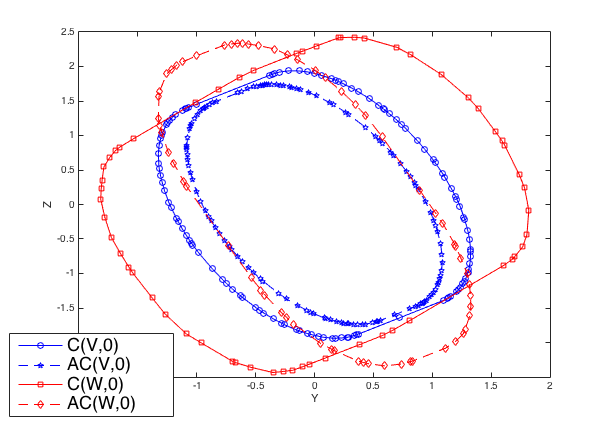
\includegraphics[scale=0.5]{fig/CZtopes/refinement.png}
\caption{Violation of positive invariance and size increase after
adding a generator to the basic representation.}~\label{fig:refinement}
\end{figure}

Alternatively, to refine
a complex zonotope, we can adjust the magnitude of contribution of
each generator to the size of the set while also preserving the
positive invariance.  This way, can also add more generators and
increase approximation accuracy by adjusting the magnitudes of each
generator.  In order to conveniently perform algebraic manipulations
on the magnitude of each generator, we can explicitly specify variable
bounds on the combining coefficients.  This gives us a more general
representation, which we call as {\it template complex zonotope},
where the magnitude of each combining coefficient is bounded in its
absolute value a {\it scaling factor}.  We call the matrix whose
column vectors generate a template complex zonotope as a {\it
template}.  This representation is similar in spirit to the known
template based set
representations~\cite{Sankaranarayanan+Dang+Ivancic-08-Symbolic,DBLP:journals/lisp/Mine06}
in abstract interpretation, where for some fixed template, subsets of
metric spaces are mapped to points in a lattice.  In the case of a
template complex zonotope, for a fixed template, subsets of the
complex vector space can be mapped to the {\it scaling factors}.
%
\begin{definition}[Template complex zonotope]
Let us consider ${\ptemp\in\mat{n}{m}{\compnums}}$ called the template,
${\sfact\in\reals^m_{\geq 0}}$ called scaling factors and
${\cen\in\compnums^n}$ called the center.  Then the following is a template
complex zonotope.
%
\begin{equation}
\tcztope{\ptemp}{\cen}{\sfact}
= \set{\ptemp\zeta+\cen:~\absolute{\zeta_i}\leq \sfact_i~\forall
i\in\set{1,...,m}}.
\end{equation}
\end{definition}
In further discussion, we use the term {\it representation size} of a
template complex zonotope to refer to the size of the template matrix.
In the rest of this chapter, we consider the following notation,
unless otherwise specified.
%
\[
\ptemp\in\mat{n}{m}{\compnums},~~\cen\in\compnums^n,~~\sfact\in\reals^m_{\geq 0}.
\]
%
A template complex zonotope can be converted to the basic
representation of the complex zonotope by multiplying the diagonal
matrix of scaling factors to the template.  This is described in the
following lemma.
%
\begin{lemma}[Normalization]~\label{lem:normalization}
Let us consider ${\mu\in\compnums^m}$.
%
\begin{align*}
\text{Then}\hspace{3em}&\tcztope{\ptemp\diagonal{\mu}}{\cen}{\sfact}=\tcztope{\ptemp}{\cen}{\diagonal{\absolute{\mu}}\sfact}.~\numberthis\label{eqn:normalization}\\
\text{Therefore},\hspace{3em} & \tcztope{\ptemp}{\cen}{\sfact}=\cztope{\ptemp\diagonal{\sfact}}{\cen}.
\end{align*}
%
\end{lemma}
%
\begin{proof}
Consider a point $x\in\tcztope{\ptemp\diagonal{\mu}}{\cen}{\sfact}$,
where
%
\[
x=\cen+\ptemp\diagonal{\mu}\zeta:\absolute{\zeta}\leq\sfact.
\]
%
Let $\zeta^\pr=\diagonal{\mu}\zeta$.  Then, $x=c+\ptemp\zeta^\pr$.
We get
%
\[
\absolute{\zeta^\pr}=\diagonal{\absolute{\mu}}\absolute{\zeta}\leq\diagonal{\absolute{\mu}}\sfact.
\]

Therefore, ${x\in\tcztope{\ptemp}{\cen}{\diagonal{\mu}\sfact}}$.  This
means,
%
\[
\tcztope{\ptemp\diagonal{\mu}}{\cen}{\sfact}\subseteq\tcztope{\ptemp}{\cen}{\diagonal{\absolute{\mu}}\sfact}
\]
%
Next consider a point
$y\in\tcztope{\ptemp}{\cen}{\diagonal{\absolute{\mu}\sfact}}$ where
%
\[
y=\cen+\ptemp\epsilon:~\absolute{\epsilon}\leq
\diagonal{\absolute{\mu}}\sfact.
\]
%
Let us consider $\epsilon^\pr\in\compnums^m$, such that
%
\[\forall i\in\set{1,...,m},~~
\epsilon_i=\left\{
\begin{array}{l}
\frac{\epsilon_i}{\mu_i}~\text{if}~\mu_i\neq 0\\
0~\text{if}~\mu_i=0.
\end{array}
\right.
\]
%
We shall show that $\epsilon=\epsilon^\pr\diagonal{\mu}$, i.e., for
any $i\in\set{1,...,m}$, $\epsilon_i=\epsilon^\pr_i\mu_i$.  We prove
it in the following two cases.
\begin{enumerate}
\item Let us consider $\epsilon_i\neq 0$.  As
$\absolute{\epsilon}\leq\absolute{\diagonal{\mu_i}}\sfact$, so
  $\mu_i\neq 0$.  Therefore,
  \[
  \epsilon_i=\frac{\epsilon_i}{\mu_i}\mu_i=\epsilon^\pr_i\mu_i.
  \]
\item Let us consider $\epsilon_i=0$.  As
$\absolute{\epsilon}\leq\absolute{\diagonal{\mu_i}}\sfact$, so $\mu_i=
  0$.  This implies
  \[
  0=\epsilon=\epsilon^\pr_i\times
  0=\epsilon^\pr_i\mu_i.
  \]
  %
\end{enumerate}
%
So, we get $y=\cen+\ptemp\diagonal{\mu_i}\epsilon^\pr$.  By the definition of
$\epsilon^\pr$, we get
%
\[\forall i\in\set{1,...,m}~~
\absolute{\epsilon^\pr_i}\leq
\left\{
\begin{array}{l}
\absolute{\frac{\epsilon_i}{\mu_i}}\leq\frac{\absolute{\mu_i}\sfact_i}{\absolute{\mu_i}}=\sfact_i~\text{if}~\mu_i\neq
0\\
0~\text{if}~\mu_i=0
\end{array}
\right.
\]
%
Therefore, $\absolute{\epsilon^\pr}\leq\sfact$.  So,
$y\in\tcztope{\ptemp\diagonal{\mu}}{\cen}{\sfact}$.  Therefore,
%
\[
\tcztope{\ptemp}{\cen}{\diagonal{\absolute{\mu}}\sfact}\subseteq\tcztope{\ptemp\diagonal{\mu}}{\cen}{\sfact}.
\]
%
Combining the previous two conclusions, we get
Equation~\ref{eqn:normalization}.

By definition,
%
\begin{align*}
& \cztope{\ptemp\diagonal{\sfact}}{\cen}=\tcztope{\ptemp\diagonal{\sfact}}{\cen}{\repmat{1}{m}{1}}\\
& \%\%~~\text{by Equation~\ref{eqn:normalization}}\\
& =\tcztope{\ptemp}{\cen}{\diagonal{{\sfact}}\repmat{1}{m}{1}}=\tcz{\ptemp}{\cen}{\sfact}.~\hspace{3em}\qedhere
\end{align*}
%
\end{proof}
%


\section{Basic operations}~\label{sec:operations-tcz}
We shall now describe other operations on augmented complex zonotopes
like are linear transformation, Minkowski sum, support function and
checking inclusion.

Augmented complex zonotopes are closed under linear transformation and
Minkowski sum, as described in the following two lemmas.  This
is because an augmented complex is specified as a Minkowski sum of a template
complex zonotope and an interval zonotope, both of which are closed
under these operations.
%
\begin{lemma}[Linear transformation]
Let us consider $A\in\mat{n}{n}{\reals}$.  Then
%
\[
A\acztope{\ptemp}{\cen}{\sfact}{\stemp}{\lb}{\ub}=\acztope{A\ptemp}{A\cen}{\sfact}{A\stemp}{\lb}{\ub}.
\]
%
\end{lemma}
%
\begin{proof}
  We derive the following.
  %
  \begin{align*}
    & A\acztope{\ptemp}{\cen}{\sfact}{\stemp}{\lb}{\ub}=
    A\lt(\minsum{\tcztope{\ptemp}{\cen}{\sfact}}{\iztope{\stemp}{\lb}{\ub}}\rt)\\
    & \%\%~\text{by Lemmas~\ref{lem:lin-transform} and~\ref{lem:iz-lin-transform}}\\
    &
    = \minsum{\tcztope{A\ptemp}{A\cen}{\sfact}}{\iztope{A\stemp}{\lb}{\ub}}\\
    & = \acztope{A\ptemp}{A\cen}{\sfact}{A\stemp}{\lb}{\ub}.~~~~~~~~~~~~~\qedhere
  \end{align*}
  %
\end{proof}
%
\begin{lemma}[Minkowski sum]
The following is true.
%
\begin{align*}
& \minsum{\acztope{\ptemp}{\cen}{\sfact}{\stemp}{\lb}{\ub}}
  {\acztope{\ptemp^\pr}{\cen^\pr}{\sfact^\pr}{\stemp^\pr}{\lb^\pr}{\ub^\pr}}\\
& = \acztope
{\lt[\begin{matrix}
    \ptemp &
    \ptemp^\pr
  \end{matrix}\rt]
}
{\begin{matrix}
    \cen+\cen^\pr
  \end{matrix}
}
{\lt[\begin{matrix}
    \sfact\\
    \sfact^\pr
  \end{matrix}\rt]
}
{\lt[\begin{matrix}
    \stemp &
    \stemp^\pr
  \end{matrix}\rt]
}
{\lt[\begin{matrix}
    \lb\\
    \lb^\pr
  \end{matrix}\rt]
}
{\lt[\begin{matrix}
    \ub\\
    \ub^\pr
  \end{matrix}\rt]
}
\end{align*}
%
\end{lemma}
%
\begin{proof}
  We derive the following.
  %
  \begin{align*}
& \minsum{\acztope{\ptemp}{\cen}{\sfact}{\stemp}{\lb}{\ub}}
    {\acztope{\ptemp^\pr}{\cen^\pr}{\sfact^\pr}{\stemp^\pr}{\lb^\pr}{\ub^\pr}}\\
& =
    \minsum{\tcztope{\ptemp}{\cen}{\sfact}}{\iztope{\stemp}{\lb}{\ub}}
    \oplus\minsum{\tcztope{\ptemp^\pr}{\cen^\pr}{\sfact^\pr}}{\iztope{\stemp^\pr}{\lb^\pr}{\ub^\pr}}\\
&
    =\lt(\minsum{\tcztope{\ptemp}{\cen}{\sfact}}{\tcztope{\ptemp^\pr}{\cen^\pr}{\sfact^\pr}}\rt)
    \oplus\lt(\minsum{\iztope{\stemp}{\lb}{\ub}}{\iztope{\stemp^\pr}{\lb^\pr}{\ub^\pr}}\rt)\\
    & \%\%~\text{by Lemmas~\ref{lem:min-sum} and~\ref{lem:iz-min-sum}}\\
& = \minsum{\tcztope{\begin{bmatrix}\ptemp &
          \ptemp^\pr\end{bmatrix}}{\cen+\cen^\pr}{\begin{bmatrix}\sfact\\\sfact^\pr\end{bmatrix}}}
             {\iztope{\mymatrix{\stemp &
                   \stemp^\pr}}{\mymatrix{\lb\\\lb^\pr}}{\mymatrix{\ub\\\ub^\pr}}}\\
& =  \acztope
{\lt[\begin{matrix}
    \ptemp &
    \ptemp^\pr
  \end{matrix}\rt]
}
{\begin{matrix}
    \cen+\cen^\pr
  \end{matrix}
}
{\lt[\begin{matrix}
    \sfact\\
    \sfact^\pr
  \end{matrix}\rt]
}
{\lt[\begin{matrix}
    \stemp &
    \stemp^\pr
  \end{matrix}\rt]
}
{\lt[\begin{matrix}
    \lb\\
    \lb^\pr
  \end{matrix}\rt]
}
{\lt[\begin{matrix}
    \ub\\
    \ub^\pr
  \end{matrix}\rt]
}.~~~~~~~~~~~~~~~~~~~\qedhere            
    \end{align*}
%
\end{proof}
%
To problem of checking inclusion between two augmented complex
zonotopes can be equivalently expressed as the problem of checking
inclusion between two geometrically equivalent template complex
zonotopes.  For this, we use the following equivalence between the
real projections of an augmented complex zonotope and a template
complex zonotope.
%
\begin{lemma}~\label{lem:acz-tcz-conversion}
The following is true.
%
\begin{align*}
  \real\lt(\acztope{\ptemp}{\cen}{\sfact}{\stemp}{\lb}{\ub}\rt)
  = \real\lt(\tcztope
  {\lt[\begin{matrix}
      \ptemp &
      \stemp
    \end{matrix}\rt]
  }
  {\begin{matrix}
      \cen+\frac{\ub+\lb}{2}
    \end{matrix}
  }
  {\lt[\begin{matrix}
      \sfact\\
      \frac{\ub-\lb}{2}
    \end{matrix}\rt]
  }
  \rt).
\end{align*}
%
\end{lemma}
%
\begin{proof}
  We derive the following.
  %
  \begin{align*}
    & \real\lt(\acztope{\ptemp}{\cen}{\sfact}{\stemp}{\lb}{\ub}\rt)
    =
    \real\lt(\tcztope{\ptemp}{\cen}{\sfact}\rt)\oplus\iztope{\stemp}{\lb}{\ub}\\
    & \%\%~\text{By Lemma~\ref{lem:iz-tcz-conversion}}\\
    & =
    \real\lt(\tcztope{\ptemp}{\cen}{\sfact}\rt)\oplus\real\lt(\tcztope{\stemp}{\stemp\frac{\ub+\lb}{2}}{\frac{\ub-\lb}{2}}\rt)\\
    &
  = \real\lt(\tcztope
  {\lt[\begin{matrix}
      \ptemp &
      \stemp
    \end{matrix}\rt]
  }
  {\begin{matrix}
      \cen+\frac{\ub+\lb}{2}
    \end{matrix}
  }
  {\lt[\begin{matrix}
      \sfact\\
      \frac{\ub-\lb}{2}
    \end{matrix}\rt]
  }
  \rt).\hspace{4em}\qedhere
   \end{align*}
  %
\end{proof}
%
 In Definition~\ref{defn:inclusion-tcz} of the previous chapter, we
 introduced a partial order ``$\order$'', as a sufficient convex
 condition for checking inclusion between two template complex
 zonotopes.  We extend the relation for checking inclusion between two
 augmented complex zonotopes as follows.
%
\begin{definition}[Ordering between augmented complex zonotopes]~\label{defn:inclusion-acz}
We say that
%
\begin{align*}
& \acztope{\ptemp^\pr}{\cen^\pr}{\sfact^\pr}{\stemp^\pr}{\lb^\pr}{\ub^\pr} \order
 \acztope{\ptemp}{\cen}{\sfact}{\stemp}{\lb}{\ub}~~\text{iff}\\
& \tcztope
  {\lt[\begin{matrix}
      \ptemp^\pr &
      \stemp^\pr
    \end{matrix}\rt]
  }
  {\begin{matrix}
      \cen^\pr+\frac{\ub^\pr+\lb^\pr}{2}
    \end{matrix}
  }
  {\lt[\begin{matrix}
      \sfact^\pr\\
      \frac{\ub^\pr-\lb^\pr}{2}
    \end{matrix}\rt]
  }  
  \order
  \tcztope
  {\lt[\begin{matrix}
      \ptemp &
      \stemp
    \end{matrix}\rt]
  }
  {\begin{matrix}
      \cen+\frac{\ub+\lb}{2}
    \end{matrix}
  }
  {\lt[\begin{matrix}
      \sfact\\
      \frac{\ub-\lb}{2}
    \end{matrix}\rt]
  }.~\numberthis\label{eqn:order-acz}
\end{align*}
%
\end{definition}
%
\begin{theorem}[Inclusion-checking and partial order]~\label{thm:acz-inclusion}
All of the following is true.
\begin{enumerate}
  \item Sufficient condition for inclusion:
%
    \begin{align*}
& \acztope{\ptemp^\pr}{\cen^\pr}{\sfact^\pr}{\stemp^\pr}{\lb^\pr}{\ub^\pr}\order\acztope{\ptemp}{\cen}{\sfact}{\stemp}{\lb}{\ub}\\    
&\implies \real\lt(\acztope{\ptemp^\pr}{\cen^\pr}{\sfact^\pr}{\stemp^\pr}{\lb^\pr}{\ub^\pr}\rt)\subseteq\real\lt(\acztope{\ptemp}{\cen}{\sfact}{\stemp}{\lb}{\ub}\rt).
\end{align*}
%
\item The relation ``$\order$'' is a partial order on
  augmented complex zonotopes.
\end{enumerate}
%
\end{theorem}
%
\begin{proof}
  We derive the following.
  %
  \begin{align*}
&    \acztope{\ptemp^\pr}{\cen^\pr}{\sfact^\pr}{\stemp^\pr}{\lb^\pr}{\ub^\pr}\order\acztope{\ptemp}{\cen}{\sfact}{\stemp}{\lb}{\ub}\\
& \equivalent   \tcztope
  {\lt[\begin{matrix}
      \ptemp^\pr &
      \stemp^\pr
    \end{matrix}\rt]
  }
  {\begin{matrix}
      \cen^\pr+\frac{\ub^\pr+\lb^\pr}{2}
    \end{matrix}
  }
  {\lt[\begin{matrix}
      \sfact^\pr\\
      \frac{\ub^\pr-\lb^\pr}{2}
    \end{matrix}\rt]
  }  
  \order
  \tcztope
  {\lt[\begin{matrix}
      \ptemp &
      \stemp
    \end{matrix}\rt]
  }
  {\begin{matrix}
      \cen+\frac{\ub+\lb}{2}
    \end{matrix}
  }
  {\lt[\begin{matrix}
      \sfact\\
      \frac{\ub-\lb}{2}
    \end{matrix}\rt]
  }\\
  & \%\%~~\text{By Theorem~\ref{thm:suff-inclusion}}\\
  & \implies
  \tcztope
  {\lt[\begin{matrix}
      \ptemp^\pr &
      \stemp^\pr
    \end{matrix}\rt]
  }
  {\begin{matrix}
      \cen^\pr+\frac{\ub^\pr+\lb^\pr}{2}
    \end{matrix}
  }
  {\lt[\begin{matrix}
      \sfact^\pr\\
      \frac{\ub^\pr-\lb^\pr}{2}
    \end{matrix}\rt]
  }  
  \subseteq
  \tcztope
  {\lt[\begin{matrix}
      \ptemp &
      \stemp
    \end{matrix}\rt]
  }
  {\begin{matrix}
      \cen+\frac{\ub+\lb}{2}
    \end{matrix}
  }
  {\lt[\begin{matrix}
      \sfact\\
      \frac{\ub-\lb}{2}
    \end{matrix}\rt]
  }\\
  & \%\%~~\text{By Lemma~\ref{lem:acz-tcz-conversion}}\\
&\implies
  \real\lt(\acztope{\ptemp^\pr}{\cen^\pr}{\sfact^\pr}{\stemp^\pr}{\lb^\pr}{\ub^\pr}\rt)\subseteq\real\lt(\acztope{\ptemp}{\cen}{\sfact}{\stemp}{\lb}{\ub}\rt).
  \end{align*}
  %
Since ``$\order$'' is a partial order on template complex zonotopes,
Equation~\ref{eqn:order-acz} implies that it is also a partial order on augmented
complex zonotopes.
\end{proof}
%
\begin{remark}
We have explained for template complex zonotopes that the relation
``$\order$'' is equivalent to second order conic constraints on the
center, scaling factors and some auxillary variables.  Therefore,
according to Equation~\ref{eqn:order-acz}, the extension of ``$\order$''
to augmented complex zonotopes is equivalent to second order conic
constraints on the primary offset, scaling factors, lower and upper
interval bounds and some auxillary variables.
\end{remark}
%
The support function of an augmented complex zonotope is as an affine
expression of the primary offset, scaling factors and the upper and
lower interval bounds.  This is described in the following lemma.
%
\begin{lemma}[Support function]~\label{lem:support-acz}
Let us consider
$v\in\reals^n$.  Then
%
\begin{align*}
  & \supp{v}{\real\lt(\acztope{\ptemp}{\cen}{\sfact}{\stemp}{\lb}{\ub}\rt)}\\
  & = \real\lt(v^T\mymatrix{\ptemp &
    \stemp}\lt(\cen+\frac{\ub+\lb}{2}\rt)\rt)+\absolute{v^T\mymatrix{\ptemp & \stemp}}\mymatrix{\sfact\\\frac{\ub-\lb}{2}}.
\end{align*}
%
\end{lemma}
%
\begin{proof}
  We derive the following:
  %
  \begin{align*}
& \%\%~~\text{by Lemma~\ref{lem:acz-tcz-conversion}}\\
&
    \supp{v}{\real\lt(\acztope{\ptemp}{\cen}{\sfact}{\stemp}{\lb}{\ub}\rt)}\\
& = \supp{v}{\real\lt(\tcztope
  {\lt[\begin{matrix}
      \ptemp &
      \stemp
    \end{matrix}\rt]
  }
  {\begin{matrix}
      \cen+\frac{\ub+\lb}{2}
    \end{matrix}
  }
  {\lt[\begin{matrix}
      \sfact\\
      \frac{\ub-\lb}{2}
    \end{matrix}\rt]
  }
  \rt)}\\
    & \%\%~\text{by Lemma~\ref{lem:support-tcz}}\\
    & =\real\lt(v^T\mymatrix{\ptemp &
    \stemp}\lt(\cen+\frac{\ub+\lb}{2}\rt)\rt)+\absolute{v^T\mymatrix{\ptemp & \stemp}}\mymatrix{\sfact\\\frac{\ub-\lb}{2}}.~\hspace{2em}\qedhere
  \end{align*}
  %
\end{proof}
%




\section{Checking inclusion}~\label{sec:inclusion-tcz}
While computing positive invariants using a set representation,
ascertaining the positive invariance of a set requires deciding the
inclusion of the next reachable set inside the given set.  In the case
of complex zonotopes, we shall show that checking the exact inclusion
amounts to solving a is a non-convex optimization problem.  Therefore,
we later find a sufficient condition expressed by convex constraints
for checking the inclusion.  The convex constraints we derive later
are specifically second order conic constraints, which are described
below.
%
\begin{definition}[Second order conic constraint]
A second order conic constraint on a variable $x$ taking values in
$\reals^n$ is one of the following expressions.
\begin{enumerate}
\item $\sqnorm{Ax+b}\leq c^Tx+d$ where $A\in\mat{r}{n}{\reals}$,
  $b\in\reals^r$, $c\in\reals^n$ and $d\in\reals$.
\item $p^Tx=q$ where $p\in\reals^n$ and $q\in\reals$.
\end{enumerate}
\end{definition}
%
\begin{example}
%
An inequality like $x^2+4y^2+25z^2-3x-4y+z+3\leq 0$ is a second order
  conic constraint because it can be written as
%
\[
\norm{\mymatrix{
    1 & 0 & 0\\
    0 & 2 & 0\\
    0 & 0 & 5
}\mymatrix{x\\y\\z}}\leq \mymatrix{3 & 4 & -1}\mymatrix{x\\y\\z}+2.
\]
A linear equality like $3x+2y-4z=5$ is also a second order conic
constraint.
\end{example}
%
In the case of complex zonotope, we shall later derive a set of second
order conic constraints, which have to be collectively satisfied to
guarantee inclusion.  Given a set of second order conic constraints on
a variable $x\in\reals^n$, solving the constraints refers to finding a
value $x^*\in\reals^n$ that satisfies the constraints.  A value
$x^\pr\in\reals^n$ is called an approximate solution within a
precision $\epsilon\in\reals_{\geq 0}$ if there exists a solution
$x^*\in\reals^n$ such that $\sqnorm{x^\pr-x^*}\leq \epsilon$.  There
are tools based on interior point methods (see~\cite{grant2008cvx})
that can efficiently find approximate solutions with very high
precision to second order conic constraints (SOCC).

Checking inclusion of a single point inside a template complex
zonotope is equivalent to solving SOCC, as described below.
%
\begin{lemma}[Inclusion of a point]
Let us consider a point $x\in\compnums^n$.  Then
$x\in\tcztope{\ptemp}{\cen}{\sfact}\subset\compnums^n$ if and only if
all of the following is collectively true.
%
\begin{align}
& \exists\zeta\in\compnums^m:\nonumber\\
& \ptemp\zeta = x-c~\label{eqn:lem-point-inclusion-1}\\
& \absolute{\zeta}\leq \sfact.~\label{eqn:lem-point-inclusion-2}
\end{align}
%
\end{lemma}
%
\begin{proof}
The above result follows from the fact that any point 
$x\in\tcztope{\ptemp}{\cen}{\sfact}$ is of the form
$x=\cen+\ptemp\zeta$ for some $\zeta\in\compnums^m$ such that
$\absolute{\zeta}\leq \sfact$.
\end{proof}
%
\begin{example}
Let us consider the template complex zonotope
$\tcztope{\ptemp}{\cen}{\sfact}\subset\compnums^2$ and a point $x\in\compnums^2$,
where
%
\[
\ptemp=\mymatrix{1+\iota & 1 & 0\\1 & 0 & 1},~~\cen = \mymatrix{\iota\\ 1},~~\sfact=\mymatrix{1\\1\\1}~\text{and}~x=\mymatrix{2\iota-2\\\iota+2}.
\]
%
To prove that $x\in\tcztope{\ptemp}{\cen}{\sfact}$, let us consider
$\zeta=\mymatrix{\iota & -1 & 1}^T$.  Then we get
%
\[
\ptemp\zeta = \mymatrix{\iota-2\\\iota+1}= \mymatrix{2\iota-2\\\iota+2}-\mymatrix{\iota\\1}=x-c.
\]
%
Therefore, Equation~\ref{eqn:lem-point-inclusion-1} is satisfied.  Furthermore,
$\absolute{\zeta}=\mymatrix{1 & 1 & 1}^T$.  So, Equation~\ref{eqn:lem-point-inclusion-2} is
also satisfied.  Henceforth, $x\in\tcztope{\ptemp}{\cen}{\sfact}$.
\end{example}
%
Equation~\ref{eqn:lem-point-inclusion-1} is an equality constraint on
$\zeta$, which is therefore an SOCC.  We know that the absolute value
of a complex number is the square norm of a two dimensional vector.
So, Equation~\ref{eqn:lem-point-inclusion-2} is equivalent to a set of
square norm constraints on the real and imaginary components of
$\zeta$, which are therefore SOCC constraints.  Hence, the inclusion
of a point inside a template complex zonotope can be checked by
solving second order conic constraints.

Now we state the necessary and sufficient condition for checking
inclusion between two template complex zonotopes.
%
\begin{lemma}[Exact inclusion between template complex zonotopes]~\label{lem:exact-inclusion}
Let us consider $\ptemp\in\mat{n}{m}{\compnums}$ and
$\ptemp^\pr\in\mat{n}{r}{\compnums}$.  The inclusion
$\tcztope{\ptemp^\pr}{\cen^\pr}{\sfact^\pr}\subseteq\tcztope{\ptemp}{\cen}{\sfact}$
holds if and only if
\begin{equation}\label{eqn:exact-inclusion}
\max_{\set{\zeta^\pr\in\compnums^{r}:\absolute{\zeta^\pr}\leq \sfact^\pr}}\min_{\set{\zeta\in\compnums^m:\ptemp\zeta=\ptemp^\pr\zeta^\pr+\cen^\pr-\cen}}\max_{i=1}^m\lt(\absolute{\zeta_i}-s_i\rt)\leq 0
\end{equation}
\end{lemma}
%
\begin{proof}
  We have
  %
  \begin{align*}
    &\tcztope{\ptemp}{\cen}{\sfact}=\set{\cen+\ptemp\zeta:~\zeta\in\compnums^m,~\absolute{\zeta}\leq\sfact},\\
    &\tcztope{\ptemp^\pr}{\cen^\pr}{\sfact^\pr}=\set{\cen^\pr+\ptemp^\pr\zeta^\pr:~\zeta^\pr\in\compnums^r,~\absolute{\zeta^\pr}\leq\sfact^\pr}.
  \end{align*}
  %
Therefore, we get
$\tcztope{\ptemp^\pr}{\cen^\pr}{\sfact^\pr}\subseteq\tcztope{\ptemp}{\cen}{\sfact}$
if and only if
for every $\zeta^\pr\in\compnums^r:\absolute{\zeta^\pr}\leq \sfact^\pr$,
there exists
$\zeta\in\compnums^m:\ptemp\zeta+\cen=\ptemp^\pr\zeta^\pr+\cen^\pr~\wedge~\absolute{\zeta}\leq
\sfact$.  This is equivalently expressed as the constraint in Equation~\ref{eqn:exact-inclusion}.
\end{proof}
%
The reason solving Equation~\ref{eqn:exact-inclusion}
requires non-convex optimization is explained as follows.  Let us consider
that $\ptemp$ has a pseudo-inverse $\pinv{\ptemp}$.  Then by the
rank-nullity theorem
%
\[
\set{\zeta:~\ptemp\zeta=\ptemp\zeta^\pr+\cen^\pr-\cen}=\set{\pinv{\ptemp}\lt(\zeta^\pr-c\rt)+v:~v\in\nullspace{\ptemp}}
\]
%
So,
%
\begin{align*}
& \min_{\set{\zeta\in\compnums:\ptemp\zeta=\ptemp^\pr\zeta^\pr+\cen^\pr-\cen}}\max_{i=1}^m\lt(\absolute{\zeta_i}-s_i\rt)\\
&
=\min_{\set{v\in\nullspace{\ptemp}}}\max_{i=1}^m\lt(\absolute{\pinv{\ptemp}\lt(\zeta^\pr-c\rt)+v}-s_i\rt)
\end{align*}
%
The absolute value of a complex variable is a convex quadratic
function of the real and imaginary components of the variable.  So,
the above function is a point-wise minimum (for points $v$ in the null
space $\null{\ptemp}$) of a set of convex quadratic functions over
$\zeta^\pr$, which is therefore a non-concave function of $\zeta^\pr$.
So the maximization
%
\[
\max_{\set{\zeta^\pr\in\compnums^{r}:\absolute{\zeta^\pr}\leq \sfact^\pr}}\min_{\set{\zeta\in\compnums^m:\ptemp\zeta=\ptemp^\pr\zeta^\pr+\cen^\pr-\cen}}\max_{i=1}^m\lt(\absolute{\zeta_i}-s_i\rt)
\]
%
is equivalent to maximizing a non-concave function of $\zeta^\pr$.
Maximizing a non-concave function is a non-convex optimization problem.

Alternatively, we shall now derive a sufficient condition, equivalent
to a set of second order conic constraints, for checking inclusion
between two template complex zonotopes.  The following result is used
to later derive the sufficient condition.
%
\begin{lemma}~\label{lem:transfer-matrix}
  Let us consider ${\sfact\in\reals^m_{\geq 0}}$,
  ${\sfact^\pr\in\reals^r_{\geq 0}}$, ${\zeta^\pr\in\compnums^r}$,
  ${\cen,\cen^\pr\in\compnums^n}$,${\ptemp\in\mat{n}{m}{\compnums}}$, ${\ptemp^\pr\in\mat{n}{r}{\compnums}}$ 
  ${\absolute{\zeta^\pr}\leq\sfact^\pr}$,
  ${\tmat\in\mat{m}{r}{\compnums}}$  and ${y\in\compnums^m}$ such that
  %
  \begin{align*}
&
    \ptemp\tmat=\ptemp^\pr\diagonal{\sfact^\pr},\hspace{1em}\ptemp\tvect=\lt(c^\pr-c\rt).~\numberthis\label{eqn:inclusion1}
    \\
&\text{Then}\hspace{2em}\min_{\set{\zeta\in\compnums:\ptemp\zeta=\ptemp^\pr\zeta^\pr+\cen^\pr-\cen}}\max_{i=1}^m\lt(\absolute{\zeta_i}-\sfact_i\rt)\leq \max_{i=1}^m\lt(\absolute{\tvect_i}+\sum_{j=1}^r\absolute{\tmat_{ij}}-\sfact_i\rt).~\numberthis\label{eqn:transfer-matrix}
\end{align*}
%
\end{lemma}
%
\begin{proof}
  Let us consider $\epsilon\in\compnums^{r}$, such that for any $i\in\set{1,...,r}$,
%
\[\left\{
\begin{array}{l}
\epsilon_i=\frac{\zeta^\pr}{s^\pr_i}~\text{if}~ s^\pr_i\neq 0\\
\epsilon_i=0~\text{otherwise}
\end{array}
\right..\]
%
From the above definition and the fact that $\absolute{\zeta^\pr}\leq
s^\pr$, we get $\zeta^\pr=\diagonal{s^\pr}\epsilon$ and
$\max_{j=1}^r\absolute{\epsilon_j}\leq 1$.  Then we derive
%
\begin{align*}
&\ptemp^\pr\zeta^\pr+c-c^\pr
=\ptemp^\pr\diagonal{\sfact^\pr}\epsilon+c-c^\pr
=\ptemp\tmat\epsilon+\ptemp\tvect
=\ptemp\lt(\tmat\epsilon+\tvect\rt)
\end{align*}
%
According the above equation,
%
\begin{align*}
& \tmat\epsilon+\tvect\in\set{\zeta\in\compnums:\ptemp\zeta=\ptemp^\pr\zeta^\pr+\cen^\pr-\cen}.\\
& \implies
  \min_{\set{\zeta\in\compnums:\ptemp\zeta=\ptemp^\pr\zeta^\pr+\cen^\pr-\cen}}\max_{i=1}^m\lt(\absolute{\zeta_i}-\sfact_i\rt)\leq
  \max_{i=1}^m\lt(\absolute{\lt(X\epsilon+y\rt)_i}-\sfact_i\rt)\\
&   ~~\%\%~\text{Using triangular inequality}\\
&\leq \max_{i=1}^m\lt(\absolute{\tvect_i}+\sum_{j=1}^r\absolute{\tmat_{ij}}\absolute{\epsilon_j}-\sfact_i\rt)\\
& ~~\%\%~\text{Since}~\max_{j=1}^r\absolute{\epsilon_j}\leq 1\\
& \leq  \max_{i=1}^m\lt(\absolute{\tvect_i}+\sum_{j=1}^r\absolute{\tmat_{ij}}-\sfact_i\rt).\hspace{3em}\qedhere
\end{align*}
%
\end{proof}
%
We define the following relation between two template
complex zonotopes, which we shall prove is a sufficient condition for
the inclusion between them.
%
\begin{definition}[Relation for inclusion-checking]~\label{defn:inclusion-tcz}
Let us consider $\ptemp\in\mat{n}{m}{\compnums}$ and
$\ptemp^\pr\in\mat{n}{r}{\compnums}$.  We say
$\tcztope{\ptemp}{\cen}{\sfact}\order\tcztope{\ptemp^\pr}{\cen^\pr}{\sfact^\pr}$
iff all of the following is collectively true.
%
\begin{align*}
& \exists \tmat\in\mat{m}{r}{\compnums},\tvect\in\compnums^m~~\text{such
that}\\
& \ptemp\tmat=\ptemp^\pr\diagonal{\sfact^\pr},~~\ptemp\tvect=\cen^\pr-\cen~\numberthis\label{eqn:inclusion-tcz1}\\
& \max_{i=1}^m\lt(\absolute{\tvect_i}+\sum_{j=1}^r\absolute{\tmat_{ij}}-\sfact_i\rt)\leq
0~\numberthis\label{eqn:inclusion-tcz2}.
\end{align*}
%
\end{definition}
%
\begin{theorem}[Inclusion checking]~\label{thm:suff-inclusion}
 If 
 ${\tcztope{\ptemp}{\cen}{\sfact}\order\tcztope{\ptemp^\pr}{\cen^\pr}{\sfact^\pr}}$
 then\\
${\tcztope{\ptemp}{\cen}{\sfact}\subseteq\tcztope{\ptemp^\pr}{\cen^\pr}{\sfact^\pr}}$.
%
\end{theorem}
%
\begin{proof}
The theorem follows from Lemmas~\ref{lem:exact-inclusion}
and~\ref{lem:transfer-matrix}.  By
Lemma~\ref{lem:exact-inclusion}, the inclusion
$\tcztope{\ptemp}{\cen}{\sfact}\subseteq\tcztope{\ptemp^\pr}{\cen^\pr}{\sfact^\pr}$
holds iff the L.H.S of Equation~\ref{eqn:exact-inclusion} is bounded
above by zero.  According to Lemma~\ref{lem:transfer-matrix}, if there
exists a $\tmat$ and $\tvect$ satisfying
Equation~\ref{eqn:inclusion1}, then the R.H.S of
Equation~\ref{eqn:transfer-matrix} is an upper bound on the L.H.S of
Equation~\ref{eqn:exact-inclusion}.  So, if there exist $\tmat$ and
$\tvect$ satisfying Equation~\ref{eqn:inclusion1} such that the R.H.S
of Equation~\ref{eqn:transfer-matrix} is bounded above by zero, then
the inclusion holds.  The relation
$\tcztope{\ptemp}{\cen}{\sfact}\order\tcztope{\ptemp^\pr}{\cen^\pr}{\sfact^\pr}$
implies that there exists $\tmat$ and $\tvect$ satisfying
Equations~\ref{eqn:inclusion1} such that the R.H.S of
Equation~\ref{eqn:transfer-matrix} is bounded above by zero.
\end{proof}
%
\begin{remark}~\label{rem:socc}
  The following constraints are equivalent to Equation~\ref{eqn:inclusion-tcz2} as
  %
  \begin{align*}
\forall
& i\in\set{1,...,m}, \exists ~a_i,b_i\\
& ~\norm{\mymatrix{\real\lt(X^T_i\rt)\\\img\lt(X^T_i\rt)}}\leq a_i, \hspace{2em}
\norm{\mymatrix{\real\lt(y_i\rt)\\\img\lt(y_i\rt)}}\leq b_i, \hspace{2em}
 0\leq \sfact_i-a_i-b_i.
\end{align*}
%
  The above is equivalent to $3m$ second order conic constraints on a
  \emph{real vector} of size at most $2mr$, which comprises the
  scaling factors and the additional variables.  Next, for a fixed
  template, Equation~\ref{eqn:inclusion-tcz1} is a set of $n(n+1)$
  linear constraints on a \emph{complex vector} of size at most
  $mr+2m+r$, which comprises the center, scaling factors and the
  additional variables.  On the other hand, the representation size of
  both the template complex zonotopes together is $(m+r)n$.
  Therefore, the size of the second order conic program for checking
  the inclusion between two template complex zonotopes can be at most
  of the order cubic in the size of the template complex zonotopes.
\end{remark}
%
%% Furthermore, the above relation is a partial order.
%
%% The relation ``$\order$'' is a partial order on the set of template
%% complex zonotopes, as stated in the following theorem.
%% %
%% \begin{theorem}[Partial ordering]
%% For any three template complex zonotopes\\
%% ${\tcz{\ptemp}{\cen}{\sfact},\tcz{\ptemp^\pr}{\cen^\pr}{\sfact^\pr}\text{
%%     and }\tcz{\ptemp^\dpr}{\cen^\dpr}{\sfact^\dpr}}$,
%% all of the following conditions are true.
%% %
%% \begin{enumerate}
%% \item Reflexivity:
%% $\tcz{\ptemp}{\cen}{\sfact}\order\tcz{\ptemp}{\cen}{\sfact}$.
%% \item Anti-symmetry: If~
%% $\tcz{\ptemp}{\cen}{\sfact}\order\tcz{\ptemp^\pr}{\cen^\pr}{\sfact^\pr}$
%% and
%% $\tcz{\ptemp^\pr}{\cen^\pr}{\sfact^\pr}\order\tcz{\ptemp}{\cen}{\sfact}$,
%% then
%% $\tcz{\ptemp}{\cen}{\sfact}=\tcz{\ptemp^\pr}{\cen^\pr}{\sfact^\pr}$.
%% \item Transitivity: If~
%% $\tcz{\ptemp^\pr}{\cen^\pr}{\sfact^\pr}\order\tcz{\ptemp}{\cen}{\sfact}$
%% and
%% $\tcz{\ptemp^\dpr}{\cen^\dpr}{\sfact^\dpr}\order\tcz{\ptemp^\pr}{\cen^\pr}{\sfact^\pr}$,
%% then $\tcz{\ptemp^\dpr}{\cen^\dpr}{\sfact^\dpr}\order\tcz{\ptemp}{\cen}{\sfact}$.
%% \end{enumerate}
%% %
%% \end{theorem}

%% \begin{proof}
%% We prove reflexivity, antisymmetry and transitivity separately as follows.
%% \begin{enumerate}
%% \item {\it Reflexivity}:  Let us consider
%%   %
%%   \begin{align*}
%% &  \tmat=\diagonal{\sfact}\text{ and }
%%   \tvect=\repmat{m}{1}{0}.\\
%% &\text{Then we get }~\ptemp\tmat=\ptemp\diagonal{\sfact},~~
%% \ptemp\tvect=0=c-c\text{ and }\\
%% & \max_{i=1}^m\lt(\absolute{y_i}+\sum_{j=1}^m\absolute{X_{ij}}-\sfact_i\rt)
%% =\max_{i=1}^m\lt(0+\sfact_i-\sfact_i\rt)=0\\
%% & \text{So}, \tcz{\ptemp}{\cen}{\sfact}\order\tcz{\ptemp}{\cen}{\sfact}.
%% \end{align*}
%% %
%% \item {\it Anti-symmetry}: Let us consider that
%% %
%% \begin{align*}
%% &
%% \tcz{\ptemp}{\cen}{\sfact}\order\tcz{\ptemp^\pr}{\cen^\pr}{\sfact^\pr}
%% \text{ and }
%% \tcz{\ptemp^\pr}{\cen^\pr}{\sfact^\pr}\order\tcz{\ptemp}{\cen}{\sfact}.\\
%% & \text{Then by Theorem~\ref{thm:suff-inclusion}, we get}\\ 
%% & \tcz{\ptemp}{\cen}{\sfact}\subseteq\tcz{\ptemp^\pr}{\cen^\pr}{\sfact^\pr}
%% \text{ and }
%% \tcz{\ptemp^\pr}{\cen^\pr}{\sfact^\pr}\subseteq\tcz{\ptemp}{\cen}{\sfact}\\
%% &\implies
%% \tcz{\ptemp}{\cen}{\sfact}=\tcz{\ptemp^\pr}{\cen^\pr}{\sfact^\pr}.
%% \end{align*}
%% %
%% \item {\it Transitivity:}  
%% \end{enumerate}
%% \end{proof}


When the template of the complex zonotope inside which containment is
checked is invertible, and the centers of the template complex
zonotopes are same, then the above sufficient condition for inclusion
checking is also a necessary condition.  This is described in the
following theorem.
%
\begin{theorem}
Let us consider
$\ptemp\in\mat{n}{n}{\compnums}$ and
$\ptemp^\pr\in\mat{n}{m}{\compnums}$ such that $\ptemp$ is a non-singular matrix.
Then
$\tcztope{\ptemp^\pr}{\cen^\pr}{\sfact^\pr}\subseteq\tcztope{\ptemp}{\cen}{\sfact}$
if and only if
$\tcztope{\ptemp^\pr}{\cen}{\sfact^\pr}\order\tcztope{\ptemp}{\cen}{\sfact}$.
\end{theorem}
%
\begin{proof}
By Theorem~\ref{thm:suff-inclusion}, we know that if
$\tcztope{\ptemp^\pr}{\cen}{\sfact^\pr}\order\tcztope{\ptemp}{\cen}{\sfact}$
is true,
then we get
$\tcztope{\ptemp^\pr}{\cen}{\sfact^\pr}\subseteq\tcztope{\ptemp}{\cen}{\sfact}$.
So, we have to prove the converse that if
$\tcztope{\ptemp^\pr}{\cen}{\sfact^\pr}\subseteq\tcztope{\ptemp}{\cen}{\sfact}$,
then
$\tcztope{\ptemp^\pr}{\cen}{\sfact^\pr}\order\tcztope{\ptemp}{\cen}{\sfact}$.

Let us consider
$\tcztope{\ptemp^\pr}{\cen}{\sfact^\pr}\subseteq\tcztope{\ptemp}{\cen}{\sfact}$.
Using
Lemma~\ref{lem:normalization}, we get
%
\begin{align*}
&
  \tcztope{\ptemp^\pr}{\cen}{\sfact^\pr}=\cztope{\ptemp^\pr\diagonal{\sfact^\pr}}{\cen}\subseteq\tcztope{\ptemp}{\cen}{\sfact}\\ &\equivalent~\set{\cen+\ptemp^\pr\diagonal{\sfact^\pr}\zeta^\pr:~\zeta^\pr\in\compnums^m,~\infnorm{\zeta^\pr}\leq
    1}\subseteq\set{\cen+\ptemp\zeta:~\zeta\in\compnums^n,~\absolute{\zeta}\leq
    \sfact}\\ & \%\%~\text{since}~\ptemp~\text{is non-singular}\\ 
  \equivalent&
  \set{\inv{\ptemp}\lt(\cen-\cen\rt)+\inv{\ptemp}\ptemp^\pr\diagonal{\sfact^\pr}\zeta^\pr:~\zeta^\pr\in\compnums^m,~\infnorm{\zeta^\pr}\leq
    1}\\& \subseteq
  \set{\zeta:\zeta\in\compnums^n,~\absolute{\zeta}\leq\sfact}\\
 & \equivalent~\set{\inv{\ptemp}\ptemp^\pr\diagonal{\sfact^\pr}\zeta^\pr:~\zeta^\pr\in\compnums^m,~\infnorm{\zeta^\pr}\leq
    1}\subseteq
  \set{\zeta:\zeta\in\compnums^n,~\absolute{\zeta}\leq\sfact} ~\numberthis\label{proof-necc-inc1}
\end{align*}
%
Let $\tmat=\inv{\ptemp}\ptemp^\pr\diagonal{\sfact^\pr}$ and
$\tvect=0$.  Then by
Equation~\ref{proof-necc-inc1}, we get for any $i\in\set{1,...,n}$
%
\begin{align*}
& \max_{\zeta^\pr\in\compnums^m:~\infnorm{\zeta}\leq 1}\absolute{\sum_{j=1}^m\tmat_{ij}\zeta_i}\leq\sfact_i.
\hspace{1em}\therefore \sum_{j=1}^m\absolute{\tmat_{ij}\frac{\absolute{\tmat_{ij}}}{\tmat_{ij}}}
    \leq\sfact_i\\
    & \%\%~~\text{since}~y_i=0\\
& \therefore \sum_{i=1}^n\absolute{\tmat_{ij}}  +\absolute{\tvect_i}\leq \sfact_i .~\numberthis\label{proof-necc-inc2}
\end{align*}
%
Furthermore, we have
%
\begin{align*}
&
  \ptemp\tmat=\ptemp\inv{\ptemp}\ptemp^\pr\diagonal{\sfact}=\ptemp^\pr\diagonal{\sfact^\pr}~\text{
    and }\\
& \ptemp\tvect=0=\cen-\cen.~\numberthis\label{proof-necc-inc3}      
\end{align*}
%
By Equations~\ref{proof-necc-inc2} and~\ref{proof-necc-inc3}, we get $\tcztope{\ptemp^\pr}{\cen}{\sfact^\pr}\order\tcztope{\ptemp}{\cen}{\sfact}$.
\end{proof}


